\documentclass[12pt,twoside]{article}
\usepackage[dvipsnames]{xcolor}
\usepackage{tikz,graphicx,amsmath,amsfonts,amscd,amssymb,bm,cite,epsfig,epsf,url}
\usepackage[hang,flushmargin]{footmisc}
\usepackage[colorlinks=true,urlcolor=blue,citecolor=blue]{hyperref}
\usepackage{amsthm,multirow,wasysym,appendix}
\usepackage{array,subcaption} 
% \usepackage[small,bf]{caption}
\usepackage{bbm}
\usepackage{pgfplots}
\usetikzlibrary{spy}
\usepgfplotslibrary{external}
\usepgfplotslibrary{fillbetween}
\usetikzlibrary{arrows,automata}
\usepackage{thmtools}
\usepackage{blkarray} 
\usepackage{textcomp}
\usepackage[left=0.8in,right=1.0in,top=1.0in,bottom=1.0in]{geometry}

%% Probability operators and functions
%
% \def \P{\mathrm{P}}
\def \P{\mathrm{P}}
\def \E{\mathrm{E}}
\def \Var{\mathrm{Var}}
\let\var\Var
\def \Cov {\mathrm{Cov}} \let\cov\Cov
\def \MSE {\mathrm{MSE}} \let\mse\MSE
\def \sgn {\mathrm{sgn}}
\def \R {\mathbb{R}}
\def \C {\mathbb{C}}
\def \N {\mathbb{N}}
\def \Z {\mathbb{Z}}
\def \cV {\mathcal{V}}
\def \cS {\mathcal{S}}

\newcommand{\RR}{\ensuremath{\mathbb{R}}}

\DeclareMathOperator*{\argmin}{arg\,min}
\DeclareMathOperator*{\argmax}{arg\,max}
\newcommand{\red}[1]{\textcolor{red}{#1}}
\newcommand{\blue}[1]{\textcolor{blue}{#1}}
\newcommand{\green}[1]{\textcolor{ForestGreen}{ #1}}
\newcommand{\fuchsia}[1]{\textcolor{RoyalPurple}{ #1}}

\newcommand{\wrnd}[1]{\widetilde{ #1 } }
\newcommand{\po}{\wrnd{\op{po}}  }

%
%% Probability distributions
%
%\def \Bern    {\mathrm{Bern}}
%\def \Binom   {\mathrm{Binom}}
%\def \Exp     {\mathrm{Exp}}
%\def \Geom    {\mathrm{Geom}}
% \def \Norm    {\mathcal{N}}
%\def \Poisson {\mathrm{Poisson}}
%\def \Unif    {\mathrm {U}}
%
\DeclareMathOperator{\Norm}{\mathcal{N}}

\newcommand{\bdb}[1]{\textcolor{red}{#1}}

\newcommand{\ml}[1]{\mathcal{ #1 } }
\newcommand{\wh}[1]{\widehat{ #1 } }
\newcommand{\wt}[1]{\widetilde{ #1 } }
\newcommand{\conj}[1]{\overline{ #1 } }
\newcommand{\rnd}[1]{\tilde{ #1 } }
\newcommand{\rv}[1]{ \rnd{ #1}  }
\newcommand{\rM}{\rnd{ m}  }
\newcommand{\rx}{\rnd{ x}  }
\newcommand{\ry}{\rnd{ y}  }
\newcommand{\rz}{\rnd{ z}  }
\newcommand{\ra}{\rnd{ a}  }
\newcommand{\rb}{\rnd{ b}  }
\newcommand{\rt}{\rnd{ t}  }
\newcommand{\rs}{\rnd{ s}  }


\newcommand{\rpc}{\widetilde{ pc}  }
\newcommand{\rndvec}[1]{\vec{\rnd{#1}}}

\def \cnd {\, | \,}
\def \Id { I }
\def \J {\mathbf{1}\mathbf{1}^T}

\newcommand{\op}[1]{\operatorname{#1}}
\newcommand{\setdef}[2]{ := \keys{ #1 \; | \; #2 } }
\newcommand{\set}[2]{ \keys{ #1 \; | \; #2 } }
\newcommand{\sign}[1]{\op{sign}\left( #1 \right) }
\newcommand{\trace}[1]{\op{tr}\left( #1 \right) }
\newcommand{\tr}[1]{\op{tr}\left( #1 \right) }
\newcommand{\inv}[1]{\left( #1 \right)^{-1} }
\newcommand{\abs}[1]{\left| #1 \right|}
\newcommand{\sabs}[1]{| #1 |}
\newcommand{\keys}[1]{\left\{ #1 \right\}}
\newcommand{\sqbr}[1]{\left[ #1 \right]}
\newcommand{\sbrac}[1]{ ( #1 ) }
\newcommand{\brac}[1]{\left( #1 \right) }
\newcommand{\bbrac}[1]{\big( #1 \big) }
\newcommand{\Bbrac}[1]{\Big( #1 \Big)}
\newcommand{\BBbrac}[1]{\BIG( #1 \Big)}
\newcommand{\MAT}[1]{\begin{bmatrix} #1 \end{bmatrix}}
\newcommand{\sMAT}[1]{\left(\begin{smallmatrix} #1 \end{smallmatrix}\right)}
\newcommand{\sMATn}[1]{\begin{smallmatrix} #1 \end{smallmatrix}}
\newcommand{\PROD}[2]{\left \langle #1, #2\right \rangle}
\newcommand{\PRODs}[2]{\langle #1, #2 \rangle}
\newcommand{\der}[2]{\frac{\text{d}#2}{\text{d}#1}}
\newcommand{\pder}[2]{\frac{\partial#2}{\partial#1}}
\newcommand{\derTwo}[2]{\frac{\text{d}^2#2}{\text{d}#1^2}}
\newcommand{\ceil}[1]{\lceil #1 \rceil}
\newcommand{\Imag}[1]{\op{Im}\brac{ #1 }}
\newcommand{\Real}[1]{\op{Re}\brac{ #1 }}
\newcommand{\norm}[1]{\left|\left| #1 \right|\right| }
\newcommand{\norms}[1]{ \| #1 \|  }
\newcommand{\normProd}[1]{\left|\left| #1 \right|\right| _{\PROD{\cdot}{\cdot}} }
\newcommand{\normTwo}[1]{\left|\left| #1 \right|\right| _{2} }
\newcommand{\normTwos}[1]{ \| #1  \| _{2} }
\newcommand{\normZero}[1]{\left|\left| #1 \right|\right| _{0} }
\newcommand{\normTV}[1]{\left|\left| #1 \right|\right|  _{ \op{TV}  } }% _{\op{c} \ell_1} }
\newcommand{\normOne}[1]{\left|\left| #1 \right|\right| _{1} }
\newcommand{\normOnes}[1]{\| #1 \| _{1} }
\newcommand{\normOneTwo}[1]{\left|\left| #1 \right|\right| _{1,2} }
\newcommand{\normF}[1]{\left|\left| #1 \right|\right| _{\op{F}} }
\newcommand{\normLTwo}[1]{\left|\left| #1 \right|\right| _{\ml{L}_2} }
\newcommand{\normNuc}[1]{\left|\left| #1 \right|\right| _{\ast} }
\newcommand{\normOp}[1]{\left|\left| #1 \right|\right|  }
\newcommand{\normInf}[1]{\left|\left| #1 \right|\right| _{\infty}  }
\newcommand{\proj}[1]{\mathcal{P}_{#1} \, }
\newcommand{\diff}[1]{ \, \text{d}#1 }
\newcommand{\vc}[1]{\boldsymbol{\vec{#1}}}
\newcommand{\rc}[1]{\boldsymbol{#1}}
\newcommand{\vx}{\vec{x}}
\newcommand{\vy}{\vec{y}}
\newcommand{\vz}{\vec{z}}
\newcommand{\vu}{\vec{u}}
\newcommand{\vv}{\vec{v}}
\newcommand{\vb}{\vec{\beta}}
\newcommand{\va}{\vec{\alpha}}
\newcommand{\vaa}{\vec{a}}
\newcommand{\vbb}{\vec{b}}
\newcommand{\vg}{\vec{g}}
\newcommand{\vw}{\vec{w}}
\newcommand{\vh}{\vec{h}}
\newcommand{\vbeta}{\vec{\beta}}
\newcommand{\valpha}{\vec{\alpha}}
\newcommand{\vgamma}{\vec{\gamma}}
\newcommand{\veta}{\vec{\eta}}
\newcommand{\vnu}{\vec{\nu}}
\newcommand{\rw}{\rnd{w}}
\newcommand{\rvnu}{\vc{\nu}}
\newcommand{\rvv}{\rndvec{v}}
\newcommand{\rvw}{\rndvec{w}}
\newcommand{\rvx}{\rndvec{x}}
\newcommand{\rvy}{\rndvec{y}}
\newcommand{\rvz}{\rndvec{z}}
\newcommand{\rvX}{\rndvec{X}}


\newtheorem{theorem}{Theorem}[section]
% \declaretheorem[style=plain,qed=$\square$]{theorem}
\newtheorem{corollary}[theorem]{Corollary}
\newtheorem{definition}[theorem]{Definition}
\newtheorem{lemma}[theorem]{Lemma}
\newtheorem{remark}[theorem]{Remark}
\newtheorem{algorithm}[theorem]{Algorithm}

% \theoremstyle{definition}
%\newtheorem{example}[proof]{Example}
\declaretheorem[style=definition,qed=$\triangle$,sibling=definition]{example}
\declaretheorem[style=definition,qed=$\bigcirc$,sibling=definition]{application}

%
%% Typographic tweaks and miscellaneous
%\newcommand{\sfrac}[2]{\mbox{\small$\displaystyle\frac{#1}{#2}$}}
%\newcommand{\suchthat}{\kern0.1em{:}\kern0.3em}
%\newcommand{\qqquad}{\kern3em}
%\newcommand{\cond}{\,|\,}
%\def\Matlab{\textsc{Matlab}}
%\newcommand{\displayskip}[1]{\abovedisplayskip #1\belowdisplayskip #1}
%\newcommand{\term}[1]{\emph{#1}}
%\renewcommand{\implies}{\;\Rightarrow\;}



\newcommand{\ru}{\rnd{ u}  }
\newcommand{\rd}{\rnd{ d}  }
%\newcommand{\rs}{\rnd{ s}  }
\newcommand{\ri}{\rnd{ i}  }
\newcommand{\re}{\rnd{ e}  }
\newcommand{\rQ}{\rnd{ q}  }
\newcommand{\rC}{\rnd{ c}  }

\newcommand{\red}[1]{{\leavevmode\color{red}{#1}}}
\newcommand{\blue}[1]{{\leavevmode\color{blue}{#1}}}
\usepackage{graphicx}
\begin{document}

\begin{center}
{\large{\textbf{Homework 7}} } \vspace{0.2cm}\\
Due November 6 at 11 pm
\\
\end{center}
Unless stated otherwise, justify any answers you give.
You can work in groups, but each
student must write their own solution based on their own
understanding of the problem.

When uploading your homework to Gradescope you will have to
select the relevant pages for each question.  Please submit each
problem on a separate page (i.e., 1a and~1b can be on the same page but 1
and 2 must be on different pages).  We understand that this may be
cumbersome but this is the best way for the grading team to grade your
homework assignments and provide feedback in a timely manner.  Failure
to adhere to these guidelines may result in a loss of points.
Note that it may take some time to
select the pages for your submission.  Please plan accordingly.  We
suggest uploading your assignment at least 30 minutes before the deadline
so you will have ample time to select the correct pages for your
submission.  If you are using \LaTeX, consider using the minted or
listings packages for typesetting code.  
\\

\begin{enumerate}

\item (Spider on a wall) There's a spider living on a wall of your living room that has a painting behind which the spider likes to hide. Figure~\ref{fig:wall} shows a diagram of the wall; it is 10 feet high and 10 feet wide.
\begin{figure}[h]
\begin{center}
\begin{tikzpicture}
\begin{axis}[grid=major, xtick={0,2,...,10}, ytick={0,2,...,10}, xmin= -1, xmax=11, ymin=-1, ymax=11]
\addplot[ very thick] coordinates
{(0,0) (0,10) (10,10) (10,0) } --cycle;
\addplot[ fill,  lightgray] coordinates
{(4,6) (4,8) (6,8) (6,6) } --cycle;
\end{axis}
\end{tikzpicture}
\end{center}
\caption{Wall and painting (in gray).}
\label{fig:wall}
\end{figure}

After observing the spider for a while you determine that (1) it spends twice the time behind the painting than on the rest of the wall, (2) it never crawls on the painting or leaves the wall, (3) if it is not behind the painting then it is equally likely to be anywhere on the wall. Since you cannot see it behind the painting, you assume that when it is there it is also equally likely to be at any spot.

\begin{enumerate}
\item Model the position of the spider as a bivariate random variable and give its pdf.
\begin{itemize}
    \item so call $\Tilde{x}$ the horizontal position, and $\Tilde{y}$ the vertical position 
    \item we know that the cdf must integrate to one, and that from teh prompt we know that the pdf is unifrom 
    \item thus we know that are behdind the painting with area of 4 thus the value of its pdf at any point is some value c such that $4c=\frac{2}{3}$ meaning that $c=\frac{1}{6}$. 
    \item working backwards we know that the rest of the wall has an area of 96 square units over which the remianing 1/3 of the pdf is spread. thus there must be some c such that $96c=\frac{1}{3}$ meaning that $c=\frac{1}{288}$
    \item so finally we get a joint cdf of 
\begin{equation*}
f_{\Tilde{x}, \Tilde{y}}(x,y)=\begin{cases}
         \frac{1}{6} \quad &\text{if} \, x \in \{4,6\}, y\in\{6,8\} \\
         0 & \text{if }x<0\cup x>10 \cup y<0\cup y>10 \\
          \frac{1}{288} \quad &\text{otherwise} \,  \\
     \end{cases}
\end{equation*}

\end{itemize}
\item Compute the pdf of the height at which the spider is located and sketch it.
\begin{itemize}
        \item if $y\in \{0,6\}, \text{ or }  y\in \{8,10\}$ then $f_{\tilde{y}}(y)=\int_{x=0}^{10}f_{\tilde{x}, \tilde{y}}(x,y)dx=\int_{x=0}^{10}\frac{1}{288}dx=\frac{10}{288}$
        \item if $y\in \{6,8\}$ then $f_{\tilde{y}}(y)=\int_{x=0}^{10}f_{\tilde{x}, \tilde{y}}(x,y)dx=\int_{x=0}^{4}\frac{1}{288}dx+\int_{x=4}^{6}\frac{1}{6}dx+\int_{x=6}^{10}\frac{1}{288}dx=\frac{8}{288}+\frac{2}{6}=\frac{13}{36}$
        \item thus our marginal cdf of y is 
        \begin{equation*}
f_{ \Tilde{y}}(y)=\begin{cases}
         \frac{13}{36} \quad &\text{if} \,  y\in\{6,8\} \\
        \frac{10}{288} \quad &\text{if} \,  y\in\{0,6\} \cup y\in\{8,10\}  \\
         0 & \text{if } \text{otherwise}   \\
     \end{cases}
\end{equation*}

\\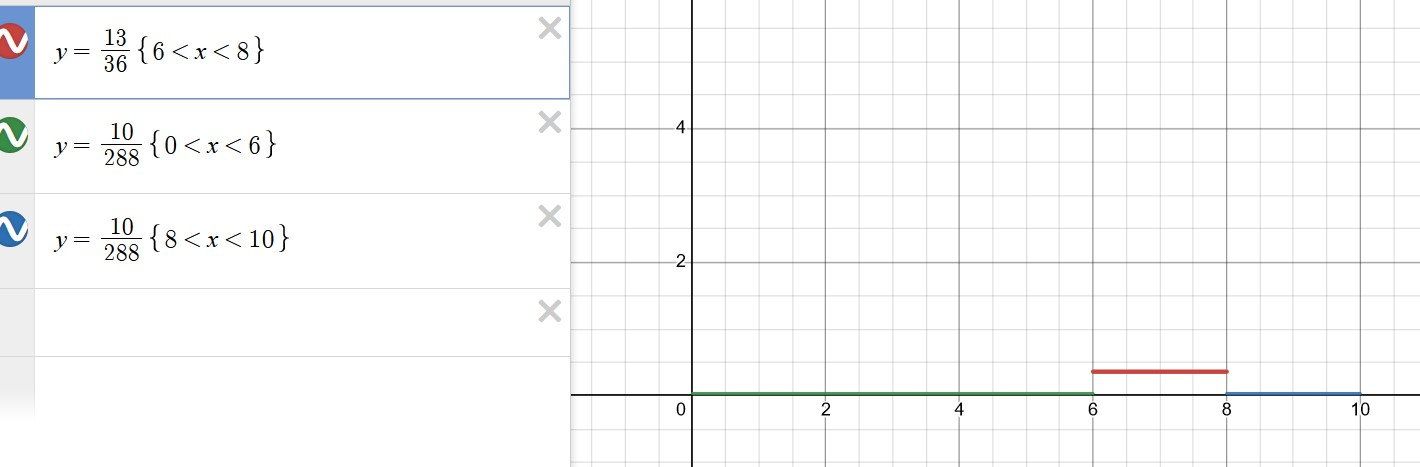
\includegraphics[width=15cm]{homework 7/1b immage.jpg}


\end{itemize}
\item Compute the conditional cdf of the height at which the spider is located, given that you can see it (i.e. it's not under the painting) and sketch it. 

\begin{itemize}
    \item let $\tilde{S}$ be a binary random variable, that takes value one if the spdier is seen. 
    \item so we are looking for $f_{\tilde{y}|\tilde{s}}(y|s=1)$
    \item notice first that $f_{\tilde{s}}(s=1)=\frac{1}{3}$ 
    \item if $y\in\{6,10\}$ then $f_{\tilde{y},\tilde{s}}(y,s=1)=\int_{0}^{10}f_{\tilde{x},\tilde{y},\tilde{s}}(x,y,s=1)dx=\int_{0}^{6}\frac{1}{288}dx+dx+\int_{8}^{10}\frac{1}{288}dx=\frac{8}{288}$
    \item meaning that for $y\in\{6,10\}$  $f_{\tilde{y}|\tilde{s}}(y|s=1)=\frac{f_{\tilde{y},\tilde{s}}(y,s=1)}{f(s=1)}=\frac{\frac{8}{288}}{\frac{1}{3}}=\frac{1}{12}$
    \item if $y\not\in\{6,10\}$ and greater than 0then $f_{\tilde{y},\tilde{s}}(y,s=1)=\int_{0}^{10}f_{\tilde{x},\tilde{y},\tilde{s}}(x,y,s=1)dx=\int_{0}^{10}\frac{1}{288}dx=\frac{10}{288}$
    \item thus for $y\not\in\{6,10\}$  that are greater than zero 
    $f_{\tilde{y}|\tilde{s}}(y|s=1)=\frac{f_{\tilde{y},\tilde{s}}(y,s=1)}{f(s=1)}=\frac{\frac{10}{288}}{\frac{1}{3}}=\frac{5}{48}$
    \item if $y\not\in\{0,10\}$ then $f_{\tilde{y},\tilde{s}}(y,s=1)=\int_{0}^{10}f_{\tilde{x},\tilde{y},\tilde{s}}(x,y,s=1)dx=\int_{0}^{10}\0dx=0$
     \item thus for $y\not\in\{0,10\}$ 
    $f_{\tilde{y}|\tilde{s}}(y|s=1)=\frac{f_{\tilde{y},\tilde{s}}(y,s=1)}{f(s=1)}=\frac{0}{\frac{1}{3}}=0$
            \item thus our conditional pdf of y on s is
        \begin{equation*}
f_{ \Tilde{y} |\tilde{s}}(y|s=1)=\begin{cases}
        \frac{1}{12} \quad &\text{if} \,  y\in\{6,8\} \\
          \frac{5}{48} \quad &\text{if} \,  y\in\{0,6\} \cup y\in\{8,10\}  \\
         0 & \text{if } \text{otherwise}   \\
     \end{cases}
\end{equation*}
\item now all that remains to do is to integrate this to get our CDF. 
\item so if $y\in \{0,6\}$ we can see that $\int_{o}^{y}f_{ \Tilde{y} |\tilde{s}}(y|s=1)=\frac{5c}{48}$
\item if $y\in \{6,8\}$ we can see that $\int_{o}^{y}f_{ \Tilde{y} |\tilde{s}}(y|s=1)=\frac{30}{48}+\frac{y-6}{12}$
\item if y$\in \{\8,10\}$ we can see that $\int_{o}^{y}f_{ \Tilde{y} |\tilde{s}}(y|s=1)=\frac{30}{48}+\frac{1}{6}+\frac{5(y-8)}{48}$
\item this fianlly yields a pdf as follows. 
        \begin{equation*}
F_{ \Tilde{y} |\tilde{s}}(y|s=1)=\begin{cases}
        0 & \text{if} y\leq 0\\
        \frac{y*5}{48} \quad &\text{if} \,  y\in\{0,6\} \\
          \frac{30}{48}+\frac{y-6}{12} \quad &\text{if} \,  y\in\{6,8\}  \\
          \frac{30}{48}+\frac{1}{6}+\frac{5(y-8)}{48} \quad &\text{if} \,  y\in\{8,10\}  \\
          1 &\text{otherwise}
     \end{cases}
\end{equation*}
\\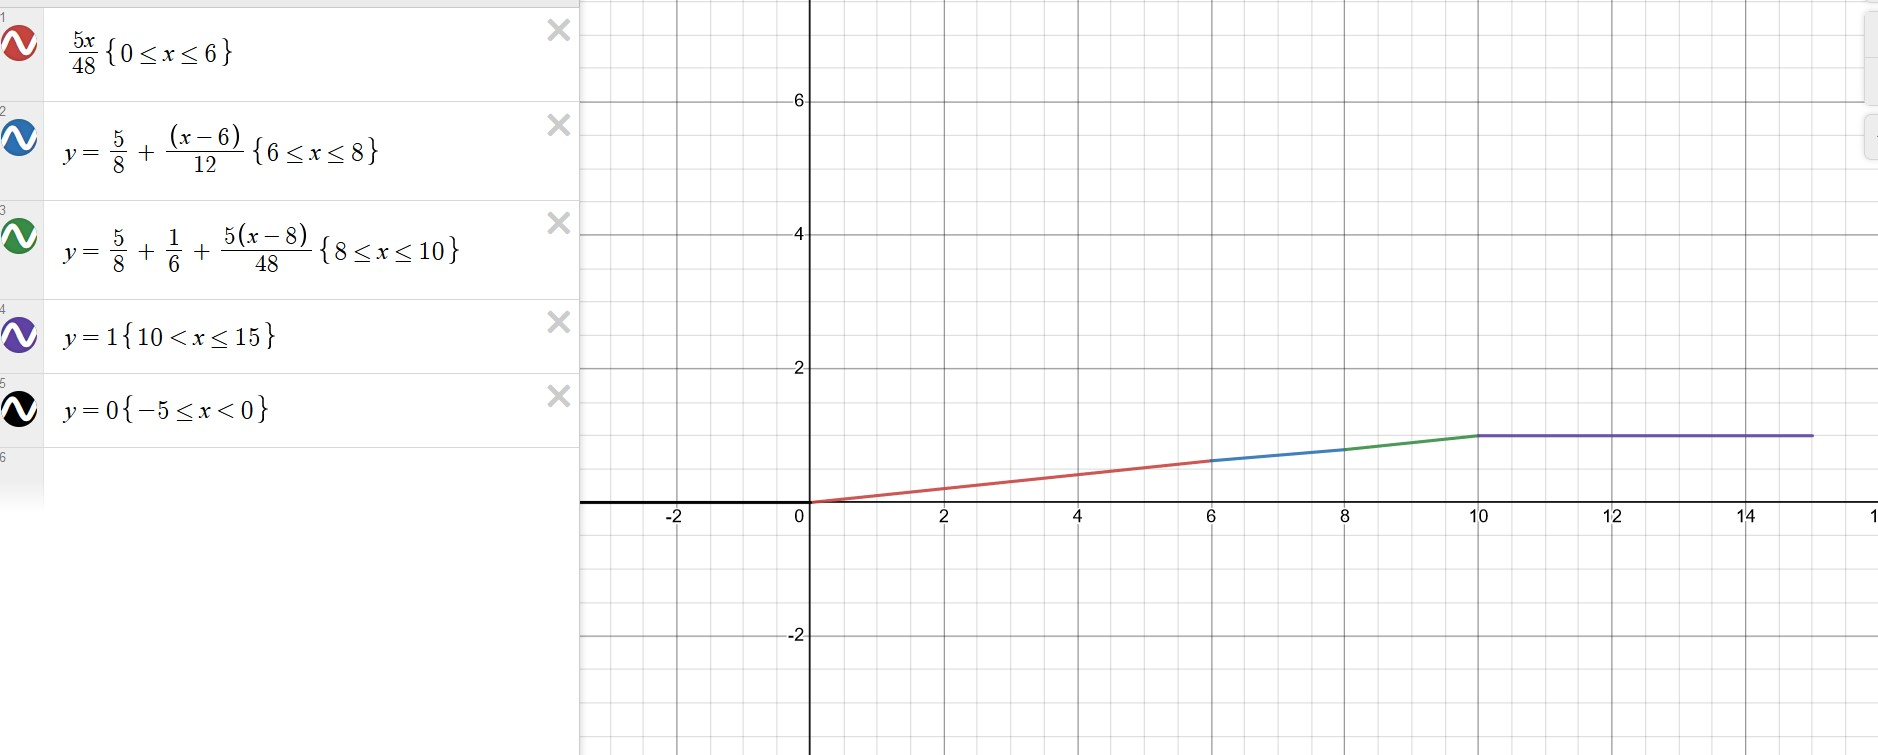
\includegraphics[width=15cm]{homework 7/1c immage.jpg}
\end{itemize}
\end{enumerate}

\item (Frog)
A frog lives in a garden where there are two ponds, see Figure~\ref{fig:garden}. It spends 1/4 of its time in the large pond and the rest in the small pond. When it is in either of the ponds, we model its position as uniformly distributed. 
\begin{enumerate}
\item What is the joint pdf of the vector that indicates the position of the frog in the diagram?


\begin{itemize}
    \item we know the joint cdf must integrate to 1. 
    \item further we know the likelyhood of the frog being anywhere but the lakes is zero
    \item thus we know the sum of the likelyood of the frog being in either point should be 1. 
    \item we know that it spends $\frac{1}{4}$ of its time in the lake. for x,y in the large lake that is $x\in\{0,10\},t\in\{0,10\}$ we can find a cconstant c such that   $,c\in\mathbb{R}:\int_{0}^{10}\int_{0}^{10}cdydx=\frac{1}{4}$ this tells us that $100c=\frac{1}{4}=P(\Tilde{x}\in\{0,10\},\Tilde{y}\in\{0,10\})=f_{\Tilde{x},\Tilde{y}}(x,y)=\frac{1}{400}$
    \item we can do the same for the small pond$x\in\{0,5\},t\in\{12,17\}$ we can find a cconstant c such that   $c\in\mathbb{R}:\int_{0}^{5}\int_{12}^{17}cdydx=\frac{3}{4}$ this tells us that $25c=\frac{3}{4}$ and thus $x\in\{0,5\},t\in\{12,17\}$ $f_{\Tilde{x},\Tilde{y}}(x,y)=\frac{3}{100}$
    \item thus our joint pdf is 
\begin{equation*}
f_{\Tilde{x},\Tilde{y}}(x,y)=\begin{cases}
          \frac{3}{100} \quad &\text{if} \, x \in \{0,5\},y \in \{12,17\} \\
                \frac{1}{400} \quad &\text{if} \, x \in \{0,10\},y \in \{0,10\} \\
                0 \quad & \text{otherwise}
     \end{cases}
\end{equation*}
\end{itemize}
\\





\item What is the marginal pdf of the horizontal position of the frog (i.e. its position on the horizontal axis)? Sketch the pdf. 
\red{
\begin{itemize}
    \item if $x\in\{0,5\}$ then $f\Tilde{x}(x)=\int_{y=0}^{17}f_{\Tilde{x},\Tilde{y}}(x,y)dy=\int_{0}^{10}\frac{1}{400}dy+\int_{12}^{17}\frac{3}{100}dy=\frac{10}{400}+\frac{15}{100}=\frac{7}{40}$
    \item if $x\in\{5,10\}$ then $f\Tilde{x}(x)=\int_{y=0}^{17}f_{\Tilde{x},\Tilde{y}}(x,y)dy=\int_{0}^{10}\frac{1}{400}dy=\frac{10}{400}=\frac{1}{40}$
        \item thus our marginal pdf is 
\begin{equation*}
f_{\Tilde{x}}(x)=\begin{cases}
          \frac{7}{40} \quad &\text{if} \, x \in \{0,5\} \\
                \frac{1}{40} \quad &\text{if} \, x \in \{5,10\}\\
                0 \quad & \text{otherwise}
     \end{cases}
\end{equation*}
\end{itemize}
}
\\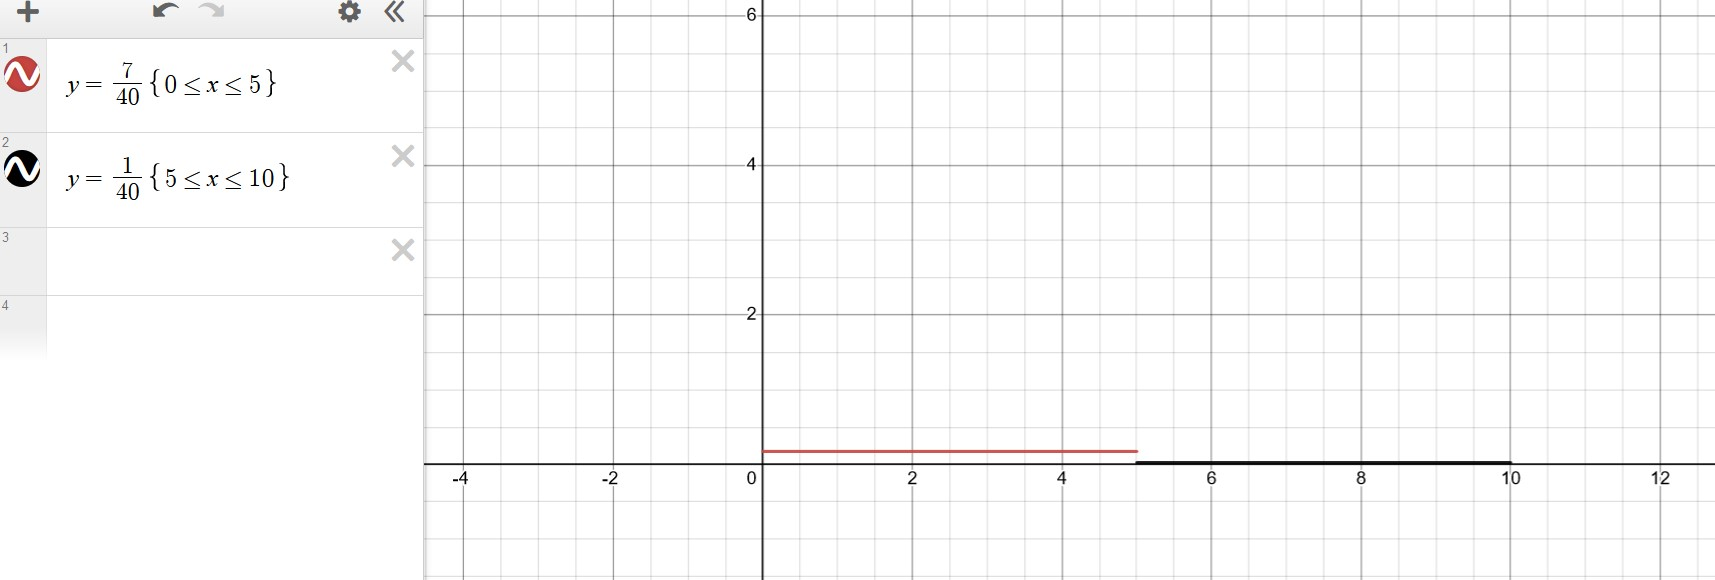
\includegraphics[width=15cm]{homework 7/question 2b.jpg}



\item If we know that the horizontal position of the frog is 3, what is the conditional pdf of its vertical position given this information? Sketch the pdf. 

\begin{itemize}
    \item if $y\in{0,10}$ then $f_{\Tilde{y}|\Tilde{x}}(y|x=3)=\frac{f_{\Tilde{y},\Tilde{x}}(y,x=3)}{f_{\Tilde{x}}(x=3)}=\frac{\frac{1}{400}}{\frac{7}{40}}=\frac{1}{70}$
        \item if $y\in{12,17}$ then $f_{\Tilde{y}|\Tilde{x}}(y|x=3)=\frac{f_{\Tilde{y},\Tilde{x}}(y,x=3)}{f_{\Tilde{x}}(x=3)}=\frac{\frac{3}{100}}{\frac{7}{40}}=\frac{1}{70}=\frac{12}{70}$
        \item thus our conditional cdf is 
    \begin{equation*}
f_{\Tilde{y}|\Tilde{x}}(y|x=3)=\begin{cases}
          \frac{1}{70} \quad &\text{if} \, y \in \{0,10\} \\
                \frac{12}{70} \quad &\text{if} \, y \in \{12,15\}\\
                0 \quad & \text{otherwise}
     \end{cases}
\end{equation*}
\\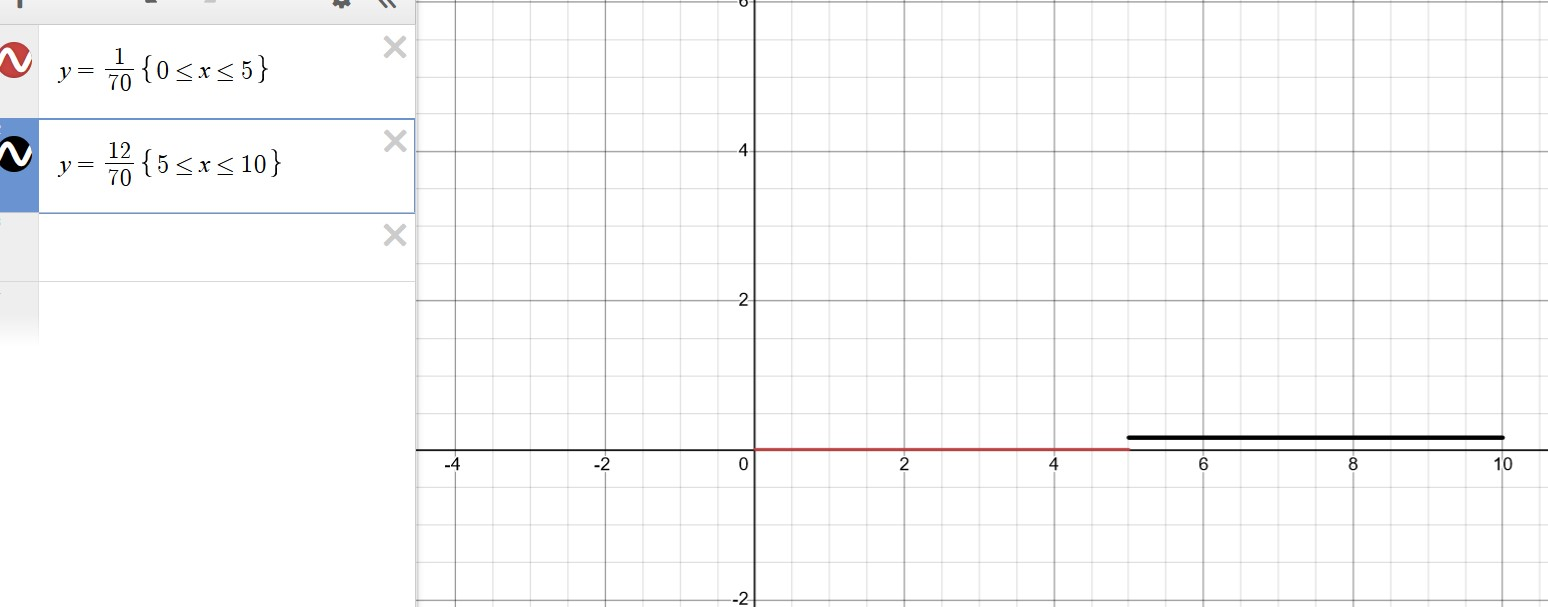
\includegraphics[width=15cm]{homework 7/question 2c.jpg}
\end{itemize}




\item Is the vertical position of the frog independent from the horizontal position of the frog? Justify your answer mathematically. 
\begin{itemize}
    \item no $\Tilde{x}, \Tilde{y}$ are not independint 
    \item to show this notice that when $y\in\{0,10\}$ $f_{\Tilde{y}}(y)=\int_{0}^{10}f(x,y)dx=\int_{0}^{10}\frac{1}{400}=\frac{1}{40}$
    \item to show this notice that when $y\in\{12,17\}$ $f_{\Tilde{y}}(y)=\int_{0}^{10}f(x,y)dx=\int_{0}^{5}\frac{15}{100}=\frac{3}{20}$
    \item so the marginal distribution of y is 
        \begin{equation*}
f_{\Tilde{y}}(y)=\begin{cases}
          \frac{1}{40} \quad &\text{if} \, y \in \{0,10\} \\
                \frac{3}{20} \quad &\text{if} \, y \in \{12,15\}\\
                0 \quad & \text{otherwise}
     \end{cases}
\end{equation*}
\item this clearly does not equal the distrobution of y conditoned on x=3, which we showed int eh last question was 
    \begin{equation*}
f_{\Tilde{y}|\Tilde{x}}(y|x=3)=\begin{cases}
          \frac{1}{70} \quad &\text{if} \, y \in \{0,10\} \\
                \frac{12}{70} \quad &\text{if} \, y \in \{12,15\}\\
                0 \quad & \text{otherwise}
     \end{cases}
\end{equation*}
\item thus $\Tilde{x},\Tilde{y}$ are not independint 
\end{itemize}

\item Is the vertical position of the frog conditionally independent from the horizontal position given the event \emph{the frog is in the small pond}? Justify your answer mathematically. 
\begin{itemize}
    \item call $\Tilde{S}$ the random vairble represneitng if the frog is in the small pond. so $P(\Tilde{s}=1)=\frac{3}{4},P(\Tilde{s}=0)=\frac{1}{4}$ 
    \item notice further that $f(x,y,s=1)=\frac{3}{100}$ as it is the liklyhood that the frog is at any point in the small point 
    \item while the marignal $f(x,s)=\int_{y=0}^{17}f(x,y,s=1)=\int_{y=12}^{17}\frac{3}{100}=\frac{15}{100}$ and the marginal$f(y,s)=\int_{x=0}^{10}f(x,y,s=1)=\int_{x=0}^{5}\frac{3}{100}=\frac{15}{100}$
    \item thus we can compute $f(x|s=1)=\frac{f(x,s=1)}{p(s=1)}=\frac{\frac{15}{100}}{\frac{3}{4}}=\frac{1}{5}=f(y|s=1)=\frac{f(y,s=1)}{p(s=1)}$ as well as $f(x,y|s=1)=\frac{f(x,y,s=1)}{p(s=1)}=\frac{\frac{3}{100}}{\frac{3}{4}}=\frac{1}{25}$
    \item thus we can see that $f(x,y|s=1)=\frac{1}{25}=\frac{1}{5}\frac{1}{5}=f(x,s)f(y,s)$ 
    \item thus x,y are indeed condtioanlly indepednint given s.
\end{itemize}


%\item Compute the mean vertical position of the frog.
% \item Consider the discrete random variable $F$ which indicates whether the frog is in the small pond or the large pond. Specify the conditional distribution of the position of the frog given $F$. 
% \item What is the mean of the position of the frog? 
\end{enumerate}
\begin{figure}[h]
\begin{center}
\begin{tikzpicture}
\begin{axis}[grid=major, xtick={0,5,10}, ytick={0,10,12,17}, xmin= -2, xmax=12, ymin=-2, ymax=19,axis on top]
\addplot[ fill, very thick, lightgray] coordinates
{(0,0) (0,10) (10,10) (10,0) } --cycle;
\addplot[fill, very thick, lightgray] coordinates
{(0,12) (0,17) (5,17) (5,12) } --cycle;
\end{axis}
\end{tikzpicture}
\end{center}
\caption{The two ponds.}
\label{fig:garden}
\end{figure}

\item (Sonar)
A scientist is trying to determine the depth of the sea at a certain location. She knows that it must be deeper than $5$ km but that is all she knows. To capture this uncertainty she models the depth as uniformly distributed between 5 and 10 km. In order to measure the depth she uses sonar, taking 2 measurements, which we model as two random variables $\rs_1$ and $\rs_2$. If the depth is equal to $x$ then each sonar measurement is uniformly distributed between $x-0.25$ and $x+0.25$. The two measurements are conditionally independent given the depth. 
\begin{enumerate}
%\item Are the two measurements independent? Justify your answer mathematically and explain it intuitively.  
\item Compute and sketch the pdf of the first sonar measurement $\rs_1$. 
\begin{itemize}
    \item we can comptue $f_{\tilde{s_1}}(s_1)=\int_{x=-\infty}^{\infty}f_{\tilde{s_1}|\tilde{x}}(s_1|x)f_{\tilde{x}}(x)dx=\int_{x=5}^{10}f_{\tilde{s_1}|\tilde{x}}(s_1|x)f_{\tilde{x}}(x)dx$
    \item now we must find $f_{\tilde{x}}$ we know that it is unifomrlaly distributed from 5,10 thus it must be the case that $f_{\tilde{x}}=c: int_{5}^{10}cdx=1$ meaning that $f_{\tilde{x}}=\frac{1}{5}$
    \item similary we can solve for $f_{\tilde{s_1}|\tilde{x}}$ as $c=f_{\tilde{s_1}|\tilde{x}}:\int_{x-.25}^{x+.25}c=\frac{1}{2}c=1$ meaning that $f_{\tilde{s_1}|\tilde{x}}=2$
    \item so if $s_1\in\{5,5.25\}$ we will have $f_{\tilde{s_1}}(s_1)=\int_{x=-\infty}^{\infty}f_{\tilde{s_1}|\tilde{x}}(s_1|x)f_{\tilde{x}}(x)dx=\int_{x=5}^{s1+.25}f_{\tilde{s_1}|\tilde{x}}(s_1|x)f_{\tilde{x}}(x)dx=\int_{x=5}^{s1+.25}f_{\tilde{s_1}|\tilde{x}}\frac{2}{5}dx=s_1\frac{2}{5}-4.75$
    \item on the other hand if $s_1\in\{5.25,9.75\}$ we will have $f_{\tilde{s_1}}(s_1)=\int_{x=-\infty}^{\infty}f_{\tilde{s_1}|\tilde{x}}(s_1|x)f_{\tilde{x}}(x)dx=\int_{x=s1-.25}^{s_1+.25}f_{\tilde{s_1}|\tilde{x}}(s_1|x)f_{\tilde{x}}(x)dx=\int_{x=s1-.25}^{s_1+.25}f_{\tilde{s_1}|\tilde{x}}\frac{2}{5}dx=\frac{1}{5}$
    \item finally we have $s_1\in\{9.75,10\}$ we will have $f_{\tilde{s_1}}(s_1)=\int_{x=-\infty}^{\infty}f_{\tilde{s_1}|\tilde{x}}(s_1|x)f_{\tilde{x}}(x)dx=\int_{x=s1-.25}^{10}f_{\tilde{s_1}|\tilde{x}}(s_1|x)f_{\tilde{x}}(x)dx=\int_{x=s1-.25}^{10}f_{\tilde{s_1}|\tilde{x}}\frac{2}{5}dx=9.75-\frac{2}{5}s1$
    \item so our final pdf is \begin{equation*}
f_{\Tilde{s_1}}{(s_1)}=\begin{cases}
          \frac{2}{5}s_1-\frac{19}{10} \quad &\text{if} \, y \in \{5,5.25\} \\
                \frac{1}{5} \quad &\text{if} \, y \in \{5.25,10\}\\
        \frac{41}{10}-\frac{2}{5}s_1 \quad &\text{if} \, y \in \{5,5.25\} \\        
                0 \quad & \text{otherwise}
     \end{cases}
\end{equation*}
    \\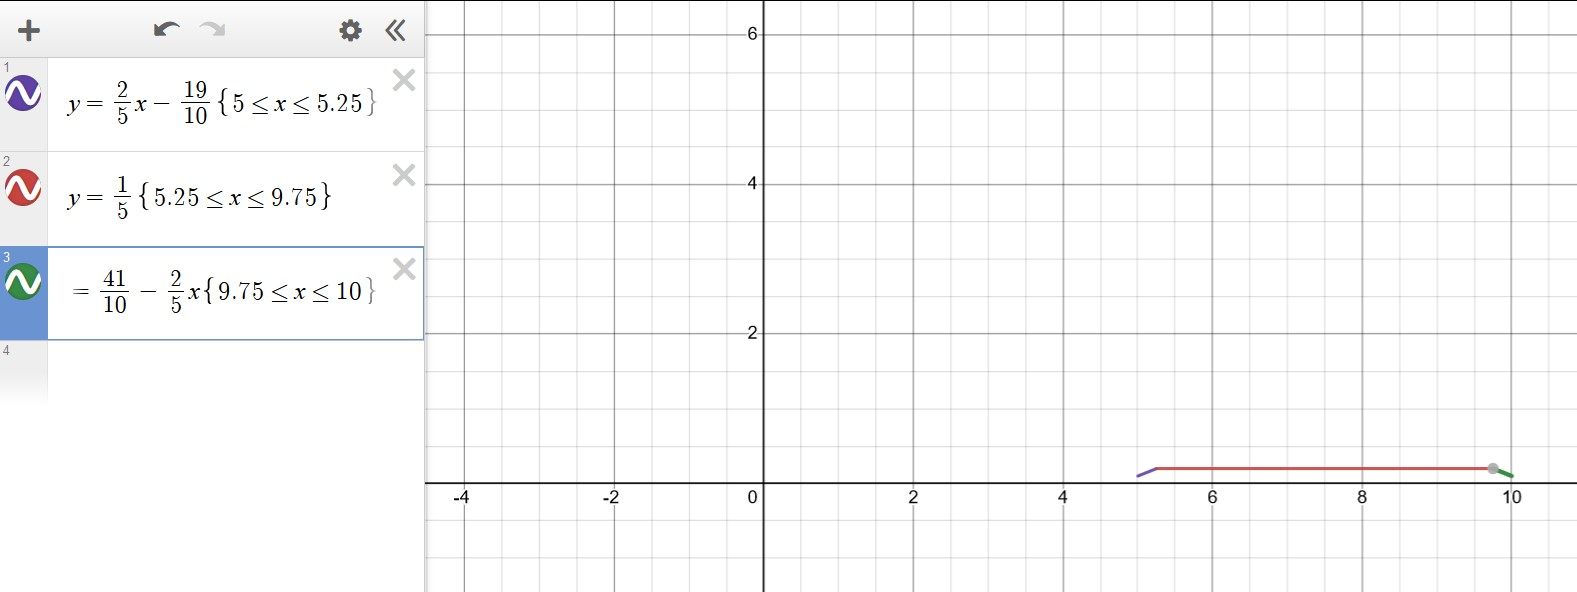
\includegraphics[width=15cm]{homework 7/question 3a.jpg}
\end{itemize}


\item Compute the conditional pdf of the depth conditioned on the measurements being equal to 7 km and 7.1 km.
\begin{itemize}
    \item we can compute $f_{\tilde{x}|\tilde{s_1},\tilde{s_1}}(x|s_1,s_2)=\frac{f(s_1,s_2|x)}{f(s_1,s_2)}=\frac{f(s_1|x)f(s_2|x)f(x)}{f(s_1,s_2)}=\frac{f(s_1|x)f(s_2|x)f(x)}{\int_{x=-\infty}^{\infty}f(s_1,s_2,x)}=\frac{f(s_1|x)f(s_2|x)f(x)}{\int_{x=-\infty}^{\infty}f(s_1|x)f(s_2|x)f(x)}$ we have computed all these terms before and we know that our numerator will only take on non zero values when x is within plus or minus .25 of both $s_1,s_2$  thus we can write $f_{\tilde{x}|\tilde{s_1},\tilde{s_1}}(x|s_1=7,s_2=7.1)=\frac{f(s_1=7|x)f(s_2=7/1|x)f(x)}{\int_{x=-\infty}^{\infty}f(s_1=7|x)f(s_2=7.1|x)f(x)}=\frac{2*2*\frac{1}{4}}{\int_{x=6.85}^{7.25}2*2*\frac{1}{5}}=\frac{5}{2}$
\end{itemize}

\item Compute the joint pdf of the two sonar measurements $\rs_1$ and $\rs_2$. Are the two measurements independent? Justify your answer mathematically and explain it intuitively.
\begin{itemize}
    \item as we briefly discussed above about joint pdf of $s_1,s_2$ is only non-zero when $s_1,s_2$ are within plus or minus .25 of one another so we can write $f(s_1,s_2)=\int_{x=-\infty}^{\infty}f(s_1,s_2,x)dx=\int_{x=-\infty}^{\infty}f(s_1|x)f(s_2|x)f(x)dx=\\\int_{min(10,s_1-.25,s_2-.25)}^{max(5,s_1+.25,s_2+.25)} f(s_1|x)f(s_2|x)f(x)dx$
    \item assume $s_1<s_2$ 
    \item if $s_1-s_2>.5$ $f(s_1,s_2)=\int_{x=-\infty}^{\infty}f(s_1,s_2,x)dx=\int_{x=-\infty}^{\infty}f(s_1|x)f(s_2|x)f(x)dx=\\\int_{min(10,s_1-.25,s_2-.25)}^{max(5,s_1+.25,s_2+.25)} f(s_1|x)f(s_2|x)f(x)dx=0$
    \item on the other hand if $s_1-s_2<.5$ $f(s_1,s_2)=\int_{x=-\infty}^{\infty}f(s_1,s_2,x)dx=\int_{x=-\infty}^{\infty}f(s_1|x)f(s_2|x)f(x)dx=\\\int_{min(10,s_1-.25,s_2-.25)}^{max(5,s_1+.25,s_2+.25)} f(s_1|x)f(s_2|x)f(x)dx=\int_{min(10,s_2-.25)}^{max(5,s_1+.25)} \frac{4}{5}dx=\frac{4}{5}(max(5,s_1+.25)-min(10,s_2-.25))$
    \item so consider a case where $s_1=.6$ and $s_2=.7$
    \item as we showed before $f(s_2=.7)=f(s_1=.6)=\frac{1}{5}$ and thus 
    \item while as $s_1-s_2=.7-.6\geq.25 f(s_1=.6,s_2=.7)=0$
    \item thus $f(s_2=.7)f(s_1=.6)=\frac{1}{5}\frac{1}{5}=\frac{1}{25}\neq 0=f(s_1=.6,s_2=.7) $
    \item thus $s_1, s_2$ are not independent 
    \item this makes senses as $s_1,s_2$ are both dependent on the depth x, and thus though they are conditionally independent if you know the distribution of just $s_1$ you are giving information about the value of the depth $x$ which will give you information about the distribution of $s_1$ 
\end{itemize}


\end{enumerate}

\item (Simulating a random vector) Explain how to simulate a random two-dimensional vector $\rx$ with a joint pdf $f_{\rx}(x)$ that is uniformly distributed in the shaded region. Assume that you have access to independent samples from a uniform distribution in $[0,1]$. Explain your method, justifying why it works. Then implement it and submit the code along with a scatterplot of 1,000 samples.


\begin{itemize}
\item we want to model dependencies within our two random variables, so we are trying to simulate draws from their joint distrobution. if we just mdoel the marginal pdfs independintly taht doe snto capture the realtionship. 
\item instead we want to take the following steps
\begin{enumerate}
    \item first we want to generate two samples form a uniform distribution between [0,1] $u_1,u_2$
    \item then we want to solve for our marginal $f_{\tilde{x}[1]}(x)$ and condtional $f_{\tilde{x}[2]|\tilde{x}[1]}(x_2|x_1)$ take there anti darivatives to get the cdfs and invert those to get $F_{\tilde{x}[1]}^{-1}(x)$ and condtional $F_{\tilde{x}[2]|\tilde{x}[1]}^{-1}(x_2|x_1)$
    \item then we first set $x=f_{\tilde{x}[1]}^{-1}(u_1)$ and use that value to compute y=$f_{\tilde{x}[2]|\tilde{x}[1]}^{-1}(x_2|x)$ allowing for the product of $x,y$ to simulate our joint cdf
\end{enumerate}
\end{itemize}



\begin{figure}[h]
\begin{center}
\begin{tikzpicture}
\begin{axis}[xtick={0,0.25,0.5,0.75,1}]%[xlabel=$x$,ylabel=$x$]
\addplot[ thick,fill, gray] coordinates
{ (0.5,1) (1,0) (0,0) } --cycle;
\end{axis}
\end{tikzpicture}
\end{center}
\end{figure}

\end{enumerate}
\end{document}
